\documentclass[12pt, aspectratio=169]{beamer}
\usetheme{madrid}
\setbeamertemplate{title page}[default][colsep=-4bp,rounded=true]
\setbeamertemplate{blocks}[rounded][shadow=false]

\usepackage[utf8]{inputenc} % this is needed for umlauts
\usepackage[ngerman]{babel} % this is needed for umlauts
\usepackage[T1]{fontenc}    % this is needed for correct output of umlauts in pdf
\usepackage{lmodern}
\usepackage{amsmath}
\usepackage{amssymb}
\usepackage{bm}
\usepackage{amsthm}
\usepackage{hyperref}
\usepackage{mdframed}
\usepackage{xcolor}
\usepackage{graphicx}
\usepackage{caption, subcaption}
\usepackage{float}
\usepackage{mathtools}

\newcommand{\Pb}{\mathbb{P}}
\newcommand{\E}{\mathbb{E}}
\newcommand{\R}{\mathbb{R}}
\newcommand{\N}{\mathbb{N}}
\newcommand{\X}{\mathbf{X}}
\newcommand{\Y}{\mathbf{Y}}
\newcommand{\T}{\bm{\Theta}}
\newcommand{\muu}{\bm{\mu}}
\newcommand{\Ssigma}{\bm{\Sigma}}
\newcommand{\vv}{\mathbf{v}}
\newcommand{\uu}{\mathbf{u}}
\newcommand{\C}{\mathbf{C}}
\newcommand{\rk}{\mathrm{rk}}
\newcommand{\A}{\mathbf{A}}
\newcommand{\B}{\mathbf{B}}
\newcommand{\Ggamma}{\bm{\Gamma}}
\newcommand{\tr}{\mathrm{tr}}
\newcommand{\xx}{\mathbf{x}}
\newcommand{\yy}{\mathbf{y}}
\newcommand{\XX}{\mathcal{X}}
\newcommand{\YY}{\mathcal{Y}}
\DeclareMathOperator*{\argmin}{argmin}

\newtheorem{ddefinition}{Definition}[section]
\newtheorem{dtheorem}[ddefinition]{Satz}
\newtheorem{dlemma}[ddefinition]{Lemma}
\newtheorem*{remark}{Bemerkung}
\newtheorem*{remarks}{Bemerkungen}


\title{Reduced-Rank-Regression}
\subtitle{Seminar Multivariate Statistik, Regression und Klassifikation}
\author{Daniel Herbst}
\date{10. Mai 2021}

\begin{document}
	
\begin{frame}[plain]
    \maketitle
\end{frame}

\begin{frame}{Gliederung}
	\tableofcontents
\end{frame}

\section{Einleitung}

\begin{frame}
	Ausgangssituation:
	$$\X := (X_1, \dots, X_r)^\top \quad \text{und} \quad \Y := (Y_1, \dots, Y_s)^\top$$
	mit gemeinsamer Verteilung $\Pb^{(\X, \Y)}$, $\Pb^\X \ll \lambda^r$, $\Pb^\Y \ll \lambda^s$ sowie $r, s \in \N$ mit $s \leq r$,
	$$ \muu_\X := \E\X, \quad \muu_\Y := \E\Y \quad \text{und} \quad \begin{pmatrix}
	\Ssigma_{\X\X} & \Ssigma_{\X\Y} \\
	\Ssigma_{\Y\X} & \Ssigma_{\Y\Y}
	\end{pmatrix} := \Ssigma \biggl(\begin{pmatrix}
	\X \\
	\Y
	\end{pmatrix}\biggr).$$
\end{frame}

\section{Klassisches multivariates Regressionsmodell mit zufälliger Inputvariable}

\begin{frame}{Das klassische lineare Regressionsmodell}
	Klassisches multivariates Regressionsmodell mit zufälliger Inputvariable:
	\[ \Y = \muu + \T \X + \mathcal{E} \text{,}\]
	wobei $\X := (X_1, \dots, X_r)^\top$ und $\Y := (Y_1, \dots, Y_s)^\top$, $s \leq r$.
	\begin{itemize}
		\item $\muu \in \R^s$ und $\T \in \R^{s \times r}$ unbekannte Parameter
		\item $\mathcal{E}$ ein (nicht beobachtbarer) $s$-dimensionaler zufälliger Fehler mit
		$$\E \mathcal{E} = 0 \quad \text{und} \quad \X \text{ und } \mathcal{E} \text{ unkorreliert.}$$
	\end{itemize}
\end{frame}

\begin{frame}{Das klassische lineare Regressionsmodell}
	Möchten optimale $\muu$ und $\T$ finden in dem Sinne, dass
	$$W(\muu, \T) := \E[(\Y - \muu - \T \X)(\Y - \muu - \T \X)^\top] \in \R^{s \times s}$$ 
	\glqq klein\grqq $\,$ wird.
	\begin{ddefinition}[Löwner-Halbordnung]
		Sei $V:= \{\A \in \R^{s \times s} \;|\; \A^\top = \A \}$ der Raum der symmetrischen $s \times s$-Matrizen.
		$$\forall \; \A, \B \in V: \; \A \leq_L \B \; :\Leftrightarrow \; \B - \A \text{ positiv semidefinit.}$$
		Es lässt sich leicht nachprüfen, dass diese Relation eine Halbordnung auf $V$, die sogenannte Löwner-Halbordnung, definiert.
	\end{ddefinition}
\end{frame}

\begin{frame}
	\begin{alertblock}{}
		\begin{center}
			Löwner-Halbordnung: $ \quad \A \leq_L \B \; :\Leftrightarrow \; \B - \A \text{ pos. semidef.}$
		\end{center}
	\end{alertblock}
	\begin{alertblock}{}
		\begin{center}
			Wollen: $ \quad W(\muu, \T) := \E[(\Y - \muu - \T \X)(\Y - \muu - \T \X)^\top] \; \rightarrow \; \min$
		\end{center}
	\end{alertblock}
$\;$ \\
	Falls $\lambda_j(\A)$ der $j$-größte Eigenwert von $\A \in \R^{s\times s}$, dann
	$$\A \leq_L \B \; \implies \; \lambda_j(\A) \leq \lambda_j(\B),  \quad j=1, \dots,s \text{.}$$
	Also:
	\[\tr(W(\muu, \T)) = \E[(\Y - \muu - \T \X)^{\top} (\Y - \muu - \T \X)] \text{,}\]
	wird ebenso minimiert.
\end{frame}

\begin{frame}
	\begin{alertblock}{}
	\begin{center}
		$W(\muu, \T) := \E[(\Y - \muu - \T \X)(\Y - \muu - \T \X)^\top] \text{,} \quad \A \leq_L \B \; :\Leftrightarrow \; \B - \A \text{ pos. semidef.}$
	\end{center}
	\end{alertblock}
	\begin{dtheorem}
		\label{thm:mr}
		In der Situation von vorher ist
		$$ \argmin_{(\muu, \T)} W(\muu, \T) = (\muu_\Y - \T_{\min} \muu_\X, \Ssigma_{\Y\X} \Ssigma_{\X\X}^{-1}) =: (\muu_{\min}, \T_{\min})  \quad \text{(bezüglich } \leq_L \text{),} $$
		$$W(\muu_{\min}, \T_{\min}) = \Ssigma_{\Y\Y} - \Ssigma_{\Y\X} \Ssigma_{\X\X}^{-1} \Ssigma_{\X\Y} \text{.}$$
		Ferner gilt für $\mathcal{E} := \Y - \muu_{\min} - \T_{\min} \X$, dass 
		$$\E \mathcal{E} = \mathbf{0} \quad \text{und} \quad \E[\mathcal{E}(\X - \muu_\X)^\top] = \mathbf{0} \text{.}$$
	\end{dtheorem}
\end{frame}

\begin{frame}
	\textit{Beweis.} $\quad$
	Mit $\X_c := \X - \muu_\X$, $\Y_c := \Y - \muu_\Y$ gilt für alle $\T \in \R^{s \times r}$, $\muu \in \R^s$:
	\begin{align*}
		W(\muu, \T) ={}& \E[(\Y - \muu - \T \X)(\Y - \muu - \T \X)^\top] \\
		={}& \E[(\Y_c - \T \X_c + (\muu_\Y - \T \muu_\X - \muu))(\Y_c - \T \X_c + (\muu_\Y - \T \muu_\X - \muu))^\top] \\
		={}& \Ssigma_{\Y\Y} - \Ssigma_{\Y\X} \T^\top - \T \Ssigma_{\X\Y} + \T \Ssigma_{\X\X} \T^\top \\
		& \quad + (\muu_\Y - \T \muu_\X - \muu)(\muu_\Y - \T \muu_\X - \muu)^\top \\
		={}& \Ssigma_{\Y\Y} - \Ssigma_{\Y\X} \Ssigma_{\X\X}^{-1} \Ssigma_{\X\Y} \\
		& \quad + \underbrace{(\Ssigma_{\Y\X} \Ssigma_{\X\X}^{-1/2} - \T \Ssigma_{\X\X}^{1/2})(\Ssigma_{\Y\X} \Ssigma_{\X\X}^{-1/2} - \T \Ssigma_{\X\X}^{1/2})^\top}_{=: A(\T) \quad \text{ positiv semidefinit}} \\
		& \quad + \underbrace{(\muu_\Y - \T \muu_\X - \muu)(\muu_\Y - \T \muu_\X - \muu)^\top}_{=:B(\muu, \T) \quad \text{positiv semidefinit}} \\
		\geq{}& \Ssigma_{\Y\Y} - \Ssigma_{\Y\X} \Ssigma_{\X\X}^{-1} \Ssigma_{\X\Y} \text{.}
	\end{align*}
\end{frame}
\begin{frame}
	\begin{alertblock}{}
		\begin{center}
			$W(\muu, \T) = \Ssigma_{\Y\Y} - \Ssigma_{\Y\X} \Ssigma_{\X\X}^{-1} \Ssigma_{\X\Y} + A(\T) + B(\muu, \T)$
		\end{center}
	\end{alertblock}
	$\implies\;$ $W(\muu, \T)$ minimal für $A(\T) = B(\muu, \T) = \mathbf{0}$, was der Fall ist, wenn
	$$ \T = \Ssigma_{\Y\X} \Ssigma_{\X\X}^{-1} =: \T_{\min} \quad \text{und} \quad \muu = \muu_\Y - \T_{\min} \muu_\X =: \muu_{\min} \text{.}$$
	Man erhält nun
	\begin{align*}
	\mathcal{E} ={}& \Y - \muu_{\min} - \T_{\min} \X \\
	={}& \Y - (\muu_\Y - (\Ssigma_{\Y\X} \Ssigma_{\X\X}^{-1}) \muu_\X) - (\Ssigma_{\Y\X} \Ssigma_{\X\X}^{-1}) \X \\
	={}& \Y_c - \Ssigma_{\Y\X} \Ssigma_{\X\X}^{-1} \X_c
	\end{align*}
	und es gilt offensichtlich $\E \mathcal{E} = \mathbf{0}$ sowie
	$$\E[\mathcal{E} \X_c^\top] = \E[(\Y_c - \Ssigma_{\Y\X} \Ssigma_{\X\X}^{-1} \X_c) \X_c^\top] = \Ssigma_{\Y\X} - \Ssigma_{\Y\X}\Ssigma_{\X\X}^{-1} \Ssigma_{\X\X} = \mathbf{0} \text{.}$$
	\hfill \qedsymbol
\end{frame}

\section{Reduced-Rank-Regressionsmodell}

\begin{frame}{Das Reduced-Rank-Regressionsmodell}
	Nun ein etwas anderes Regressionsmodell:
	\[\Y = \muu + \C \X + \mathcal{E} \text{,}\]
	wobei
	\begin{itemize}
		\item $\muu \in \R^s$ und $\C \in \R^{s \times r}$ unbekannte Parameter
		\item $\mathcal{E}$ nicht beobachtbarer, zufälliger Fehler mit $\E \mathcal{E} = 0$ und Kovarianzmatrix $\Ssigma_{\mathcal{E} \mathcal{E}}$
		\item $\X$ und $\mathcal{E}$ unkorreliert
		\item es gibt ein $t \in \{0,\dots,s\}$ mit $ \rk \, \C \leq t \leq s \text{.}$
	\end{itemize}
	In diesem Fall gibt es Matrizen $\A \in \R^{s \times t}$ und $\B \in \R^{t \times r}$ mit $\C = \A \B$, d.h. das Modell
	lässt sich auch schreiben als
	\[\Y = \muu + \A \B \X + \mathcal{E} \text{.}\]
\end{frame}

\begin{frame}
\begin{alertblock}{}
	\begin{center}
		$\Y = \muu + \C \X + \mathcal{E}\text{,} \qquad \C = \A \B \; \text{mit} \; \C \in \R^{s \times r}\text{,} \A \in \R^{s \times t} \text{,} \B \in \R^{t \times r}$
	\end{center}
\end{alertblock}
\begin{alertblock}{}
	\begin{center}
		$W(\muu, \T) := \E[(\Y - \muu - \T \X)(\Y - \muu - \T \X)^\top] \text{,} \quad \A \leq_L \B \; :\Leftrightarrow \; \B - \A \text{ pos. semidef.}$
	\end{center}
\end{alertblock}
$\;$ \\
Möchten auch hier wieder $\muu \in \R^s$, $\A \in \R^{s \times t}$ und $\B \in \R^{t \times r}$ finden, die $\Y - \muu - \A \B \X$ auf eine gewisse Art und Weise minimieren, gehen nun aber etwas anders vor: \\
	$\Ggamma \in \R^{s \times s}$ symmetrisch positiv definite Gewichtsmatrix, minimiere 
	$$ W_{t, \Ggamma}(\muu, \A, \B) := \E[(\Y - \muu - \A \B \X)^{\top} \Ggamma (\Y - \muu - \A \B \X)]$$
	über $\muu$, $\A$ und $\B$.
\end{frame}

\begin{frame}
\begin{dtheorem}
	\label{thm:rrr}
	Seien $\X$ und $\Y$ wie vorher und $0 \leq t \leq s$. Dann ist
	\begin{center}
		$\argmin_{(\muu, \A, \B)} W_{t, \Ggamma}(\muu, \A, \B) = (\muu^{(t)}_{\min}, \A^{(t)}_{\min}, \B^{(t)}_{\min}) \quad  \text{mit}$
	\end{center}
	\begin{alignat*}{3}
	&\A^{(t)}_{\min}   &&:= \Ggamma^{-1/2} \mathbf{U}_t                                       &&\quad \in \R^{s \times t} \\
	&\B^{(t)}_{\min}   &&:= \mathbf{U}_t^\top \Ggamma^{1/2} \Ssigma_{\Y\X}\Ssigma_{\X\X}^{-1} &&\quad \in \R^{t \times r} \\
	&\muu^{(t)}_{\min} &&:= \muu_\Y - \A^{(t)}_{\min} \B^{(t)}_{\min} \muu_\X                 &&\quad \in \R^s \text{,}
	\end{alignat*}
	wobei $\mathbf{U}_t := (\uu_1,\dots, \uu_t) \in \R^{s \times t}$ und $\uu_1,\dots, \uu_t$ orthonormale Eigenvektoren zu den Eigenwerten $\lambda_1 \geq \dots \geq \lambda_t \geq 0$ von $\Ggamma^{1/2} \Ssigma_{\Y\X} \Ssigma_{\X\X}^{-1} \Ssigma_{\X\Y} \Ggamma^{1/2}$ seien.
	Ferner gilt
	$$W_{t, \Ggamma}(\muu^{(t)}_{\min}, \A^{(t)}_{\min}, \B^{(t)}_{\min}) = \tr(\Ssigma_{\Y\Y}) \tr(\Ggamma) - \sum_{i=1}^{t} \lambda_i \text{.}$$
\end{dtheorem}
\end{frame}

\begin{frame}
	\begin{alertblock}{}
		\begin{center}
			Wollen: $ W_{t, \Ggamma}(\muu, \C) := \E[(\Y - \muu - \C \X)^{\top} \Ggamma (\Y - \muu - \C \X)] \; \rightarrow \; \min$
		\end{center}
	\end{alertblock}
$\;$ \\
	\textit{Beweis.} $\quad$ 
	Für $\muu \in \R^s$, $\C \in \R^{s \times r}$ und $\X_c := \X - \muu_\X$, $\Y_c := \Y - \muu_\Y$ gilt: 
	\begin{align*}
	W_{t, \Ggamma}(\muu, \C) ={}& \E[(\Y - \muu - \C \X)^\top \Ggamma (\Y - \muu - \C \X)] \\
	={}& \E[(\Y_c - \C \X_c + (\muu_\Y - \C \muu_\X - \muu))^\top \Ggamma (\Y_c - \C \X_c + (\muu_\Y - \C \muu_\X - \muu))] \\
	={}& \E[(\Y_c - \C \X_c)^\top \Ggamma (\Y_c - \C \X_c)] \\
	& \quad + \underbrace{(\muu_\Y - \C \muu_\X - \muu)^\top \Ggamma (\muu_\Y - \C \muu_\X - \muu)}_{\geq 0 \quad \text{(da } \Ggamma \text{ symmetrisch positiv definit)}}
	\end{align*}
\end{frame}

\begin{frame}
	\begin{alertblock}{}
		\begin{center}
			Wollen: $\E[(\Y_c - \C \X_c)^\top \Ggamma (\Y_c - \C \X_c)] \; \rightarrow \; \min$
		\end{center}
	\end{alertblock}
$\;$ \\
	Mit $\Ssigma_{\X\X}^\ast := \Ssigma_{\X\X}$, $\Ssigma_{\Y\Y}^\ast := \Ggamma^{1/2} \Ssigma_{\Y\Y} \Ggamma^{1/2}$, $\Ssigma_{\Y\X}^\ast := \Ggamma^{1/2} \Ssigma_{\Y\X}$, $\Ssigma_{\X\Y}^\ast := \Ssigma_{\X\Y} \Ggamma^{1/2}$ und $\C^\ast := \Ggamma^{1/2} \C$ ist
	\begin{align*}
	\E[(\Y_c - \C \X_c)^\top \Ggamma (\Y_c - \C \X_c)] ={}& \E[\Y_c^\top \Ggamma \Y_c - \X_c^\top \C^\top \Ggamma \Y_c - \Y_c^\top \Ggamma \C
	\X_c + \X_c^\top \C^\top \Ggamma \C \X_c] \\
	={}& \tr(\Ssigma_{\Y\Y}^\ast - \C^\ast \Ssigma_{\X\Y}^\ast - \Ssigma_{\Y\X}^\ast \C^{\ast
		\top} + \C^\ast \Ssigma_{\X\X}^\ast \C^{\ast \top}) \\
	={}& \tr(\Ssigma_{\Y\Y}^\ast - \Ssigma_{\Y\X}^\ast \Ssigma_{\X\X}^{\ast -1}
	\Ssigma_{\X\Y}^\ast) \\
	&+ \tr( \; (\C^\ast \Ssigma_{\X\X}^{\ast 1/2} - \Ssigma_{\Y\X}^\ast \Ssigma_{\X\X}^{\ast -1/2}) \\
	& \qquad \cdot (\C^\ast \Ssigma_{\X\X}^{\ast 1/2} - \Ssigma_{\Y\X}^\ast \Ssigma_{\X\X}^{\ast -1/2})^\top \; ).                                                  
	\end{align*}
\end{frame}

\begin{frame}
\begin{alertblock}{}
	\setlength\abovedisplayskip{0pt}
	\begin{align*}
		\E[(\Y_c - \C \X_c)^\top \Ggamma (\Y_c - \C \X_c)] ={}& \text{Konst.} 
		+ \tr( \; (\C^\ast \Ssigma_{\X\X}^{\ast 1/2} - \Ssigma_{\Y\X}^\ast \Ssigma_{\X\X}^{\ast -1/2}) \\
		&  \;\; \quad \quad \qquad \cdot (\C^\ast \Ssigma_{\X\X}^{\ast 1/2} - \Ssigma_{\Y\X}^\ast \Ssigma_{\X\X}^{\ast -1/2})^\top \;)
	\end{align*}
\end{alertblock}
\begin{dlemma}[Satz von Eckart-Young]
	Seien $\A, \B \in \R^{m \times n}$ und $b := \rk \, \B \leq \rk \, \A =: r$, und sei
	$\lambda_j(\C)$ für eine reelle symmetrische Matrix $\C$ deren $j$-größter Eigenwert.
	Dann gilt:
	$$\lambda_j((\A - \B)(\A - \B)^\top) \geq \lambda_{j+b}(\A \A^\top)$$
	mit Gleichheit für
	$$\A_b := \sum_{i=1}^{b} \lambda_i^{1/2} \mathbf{u}_i \mathbf{v}_i^\top \text{,}$$
	wobei $\lambda_i := \lambda_i(\A \A^\top)$ und $\mathbf{u}_i$ bzw. $\mathbf{v}_i$ jeweils orthonormale Eigenvektoren von $\A \A^\top$ bzw. 
	$\A^\top \A$ zu $\lambda_i$ seien.
\end{dlemma}
\end{frame}

\begin{frame}
\begin{alertblock}{}
	\setlength\abovedisplayskip{0pt}
	\begin{align*}
	\E[(\Y_c - \C \X_c)^\top \Ggamma (\Y_c - \C \X_c)] ={}& \text{Konst.} 
	+ \tr( \; (\C^\ast \Ssigma_{\X\X}^{\ast 1/2} - \Ssigma_{\Y\X}^\ast \Ssigma_{\X\X}^{\ast -1/2}) \\
	&  \;\; \quad \quad \qquad \cdot (\C^\ast \Ssigma_{\X\X}^{\ast 1/2} - \Ssigma_{\Y\X}^\ast \Ssigma_{\X\X}^{\ast -1/2})^\top \;)
	\end{align*}
\end{alertblock}
	$k:= \rk \, \Ssigma_{\Y\X} = \rk \, \Ssigma_{\Y\X}^\ast \Ssigma_{\X\X}^{\ast -1/2}$
	und seien $\uu_i$ orthonormale Eigenvektoren zu $\lambda_i$ von
	$$(\Ssigma_{\Y\X}^\ast \Ssigma_{\X\X}^{\ast -1/2})(\Ssigma_{\Y\X}^\ast \Ssigma_{\X\X}^{\ast -1/2})^\top = \Ssigma_{\Y\X}^\ast \Ssigma_{\X\X}^{\ast -1} \Ssigma_{\X\Y}^\ast = \Ggamma^{1/2} \Ssigma_{\Y\X} \Ssigma_{\X\X}^{-1} \Ssigma_{\X\Y} \Ggamma^{1/2}, \quad 1 \leq i \leq s,$$
	$$\vv_i := \lambda_i^{-1/2} \Ssigma_{\X\X}^{\ast -1/2} \Ssigma_{\X\Y}^\ast \uu_i = \lambda_i^{-1/2} \Ssigma_{\X\X}^{-1/2} \Ssigma_{\X\Y} \Ggamma^{1/2} \uu_i\text{,} \quad 1 \leq i \leq k$$
	$\xRightarrow[]{\text{Eckart-Young}}$ Zweiter Term von $(\ast)$ minimal für 
	$$\C^\ast \Ssigma_{\X\X}^{\ast 1/2} = \Ggamma^{1/2} \C \Ssigma_{\X\X}^{1/2} = \sum_{i=1}^{\min\{k, t\}} \lambda_i^{1/2} \uu_i \vv_i^\top \quad \text{also}$$
	$$\C^{(t)}_{\min} := \Ggamma^{-1/2} \biggl( \, \sum_{i=1}^{\min\{k, t\}} \lambda_i^{1/2} \uu_i \vv_i^\top \biggr) \Ssigma_{\X\X}^{-1/2}
	= \Ggamma^{-1/2} \biggl( \sum_{i=1}^{t} \uu_i \uu_i^\top \biggr) \Ggamma^{1/2} \Ssigma_{\Y\X} \Ssigma_{\X\X}^{-1} \text{.}$$
\end{frame}

\begin{frame}
	\begin{alertblock}{}
		\setlength\abovedisplayskip{0pt}
		\begin{align*}
		W_{t, \Ggamma}(\muu, \C) :={}& \E[(\Y - \muu - \C \X)^{\top} \Ggamma (\Y - \muu - \C \X)] \\
		={}& \text{Konst.} 
		+ \tr( \; (\C^\ast \Ssigma_{\X\X}^{\ast 1/2} - \Ssigma_{\Y\X}^\ast \Ssigma_{\X\X}^{\ast -1/2}) \\
		&  \;\; \quad \quad \qquad \cdot (\C^\ast \Ssigma_{\X\X}^{\ast 1/2} - \Ssigma_{\Y\X}^\ast \Ssigma_{\X\X}^{\ast -1/2})^\top \;) \\
		&+ (\muu_\Y - \C \muu_\X - \muu)^\top \Ggamma (\muu_\Y - \C \muu_\X - \muu)
		\end{align*}
	\end{alertblock}
\begin{alertblock}{}
	\begin{center}
		$\C^{(t)}_{\min} = \Ggamma^{-1/2} \biggl( \sum_{i=1}^{t} \uu_i \uu_i^\top \biggr) \Ggamma^{1/2} \Ssigma_{\Y\X} \Ssigma_{\X\X}^{-1}$
	\end{center}
\end{alertblock}
	$\implies$ $W_{t, \Ggamma}(\muu, \A, \B)$ minimal für
	\begin{alignat*}{3}
	&\A^{(t)}_{\min}   &&= \Ggamma^{-1/2} \mathbf{U}_t                                       &&\quad \in \R^{s \times t} \\
	&\B^{(t)}_{\min}   &&= \mathbf{U}_t^\top \Ggamma^{1/2} \Ssigma_{\Y\X}\Ssigma_{\X\X}^{-1} &&\quad \in \R^{t \times r} \\
	&\muu^{(t)}_{\min} &&= \muu_\Y - \A^{(t)}_{\min} \B^{(t)}_{\min} \muu_\X                 &&\quad \in \R^s \text{,}
	\end{alignat*}
	wobei $\mathbf{U}_t := (\uu_1,\dots, \uu_t) \in \R^{s \times t}$. \hfill \qedsymbol
\end{frame}

\begin{frame}{Spezialfälle der Reduced-Rank-Regression}
	\begin{alertblock}{}
		\begin{center}
			Haben soeben $ W_{t, \Ggamma}(\muu, \C) := \E[(\Y - \muu - \C \X)^{\top} \Ggamma (\Y - \muu - \C \X)]$ minimiert
		\end{center}
	\end{alertblock}
$\;$ \\
	Spezielle Wahlen von $\Ggamma$ und $\X, \Y$:
	\begin{itemize}
		\item $\X = \Y$ und $\Ggamma = \mathbf{I}_s$: \textit{Hauptkomponentenanalyse (principal component analysis, PCA)} (Vortrag 6).
		\item $\Ggamma = \Ssigma_{\Y\Y}^{-1}$: \textit{kanonische Korrelationsanalyse} (Vortrag 7).
		\item Setup der kanonischen Korrelationsanalyse für einen $\{0, 1\}$-wertigen Vektor $\Y$, der Gruppenzugehörigkeiten modelliert: \textit{lineare Diskriminanzanalyse} (Vortrag 8).
	\end{itemize}
\end{frame}

\begin{frame}{Stichprobenschätzung bei der Reduced-Rank-Regression}
	Zur Minimierung benötigt: $\muu_\X, \muu_\Y$ und $\Ssigma_{\X\X}, \Ssigma_{\X\Y}, \Ssigma_{\Y\X}, \Ssigma_{\Y\Y}$  - typischerweise unbekannt. 
	I.d.R. Stichprobe gegeben:
	\[\mathcal{D} := \{(\xx_j, \yy_j) \;|\; 1 \leq j \leq n\} \text{,}\]
	unabhängige Realisierungen von $r$- bzw. $s$-dimensionalen Zufallsvektoren $\X$ bzw. $\Y$.
	Arbeiten stattdessen einfach mit den entsprechenden empirischen Größen:
	\[\widehat{\muu}_{\X} := \frac{1}{n} \sum_{j=1}^{n} \mathbf{x}_j = \bar{\xx}_n \text{,} \quad \widehat{\muu}_{\Y} := \frac{1}{n} \sum_{j=1}^{n} \mathbf{y}_j = \bar{\yy}_n\]
	$$\xx_{cj} := \xx_j - \bar{\xx}_n \text{,} \quad \yy_{cj} := \yy_j - \bar{\yy}_n \text{,} \quad \XX_c := (\xx_{c1},\dots,\xx_{cn}) \text{,} \quad \YY_c := (\yy_{c1},\dots,\yy_{cn})$$
	$$ \widehat{\Ssigma}_{\X\X} := \frac{1}{n} \XX_c \XX_c^\top \in \R^{r \times r} \text{,} \quad \widehat{\Ssigma}_{\Y\Y} := \frac{1}{n} \YY_c \YY_c^\top \in \R^{s \times s} \text{,}$$
	\[\widehat{\Ssigma}_{\Y\X} := \frac{1}{n} \YY_c \XX_c^\top = \widehat{\Ssigma}_{\X\Y}^\top \in \R^{s \times r} \text{.}\]
\end{frame}

\begin{frame}{Stichprobenschätzung bei der Reduced-Rank-Regression}
	$$\widehat{\C}^{(t)}_{\min} := \Ggamma^{-1/2} \biggl( \sum_{i=1}^{t} \widehat{\uu}_i \widehat{\uu}_i^\top \biggr) \Ggamma^{1/2} \widehat{\Ssigma}_{\Y\X} \widehat{\Ssigma}_{\X\X}^{-1} \text{,}$$
	wobei $\widehat{\uu}_i\text{,} \; 1 \leq i \leq t$ orthonormale Eigenvektoren zu den je $i$-größten Eigenwerten $\lambda_i \text{,} \; 1 \leq i \leq t$ von
	$\Ggamma^{1/2} \widehat{\Ssigma}_{\Y\X} \widehat{\Ssigma}_{\X\X}^{-1} \widehat{\Ssigma}_{\X\Y} \Ggamma^{1/2}$ seien. $\T_{\min}$ wird analog durch
	$$\widehat{\T}_{\min} := \widehat{\Ssigma}_{\Y\X} \widehat{\Ssigma}_{\X\X}^{-1}$$
	geschätzt.
\end{frame}

\begin{frame}{Simulationsbeispiel}
	Erzeugen je $n=1000$ unabhängige Realisierungen 
	$$\xx_j \sim \mathcal{N}_3(\mathbf{0}, \; 0.3 \cdot \mathbf{I}_3)\text{,} \quad \bm{\varepsilon}_j \sim \mathcal{N}_3(\mathbf{0}, \; 0.15 \cdot \mathbf{I}_3)\text{,}\quad 1 \leq j \leq n \text{,}$$
	$$\C := \frac{1}{4} \cdot \begin{pmatrix}
	1 & 0 & 1 \\
	0 & 1 & 0 \\
	0 & 0 & -1
	\end{pmatrix} \in \R^{3 \times 3} \text{,} \quad \muu := \begin{pmatrix}
	0.5 \\
	0.5 \\
	0.5
	\end{pmatrix} \text{,} \quad \yy_j := \muu + \C \xx_j + \bm{\varepsilon}_j$$
	Stichprobe:
	\[\mathcal{D} := \{(\xx_j, \yy_j) \;|\; 1 \leq i \leq n\}\text{,}\]
	verwenden $\Ggamma := \mathbf{I}_s$ bei der Reduced-Rank-Regression.
	$$ \implies \quad \widehat{\muu}_{\min}^{(3)} \approx \begin{pmatrix}
	0.504 \\
	 0.490 \\
	  0.499
	\end{pmatrix} \text{,} \quad \widehat{\C}_{\min}^{(3)} \approx \begin{pmatrix}
	0.246 & -0.018 & 0.241 \\
	-0.018 & 0.212 & 0.007 \\
	-0.017 & -0.017 & -0.279
	\end{pmatrix}$$
\end{frame}

\begin{frame}
	\begin{figure}[H]
		\centering
		\begin{subfigure}{0.2\textwidth}
			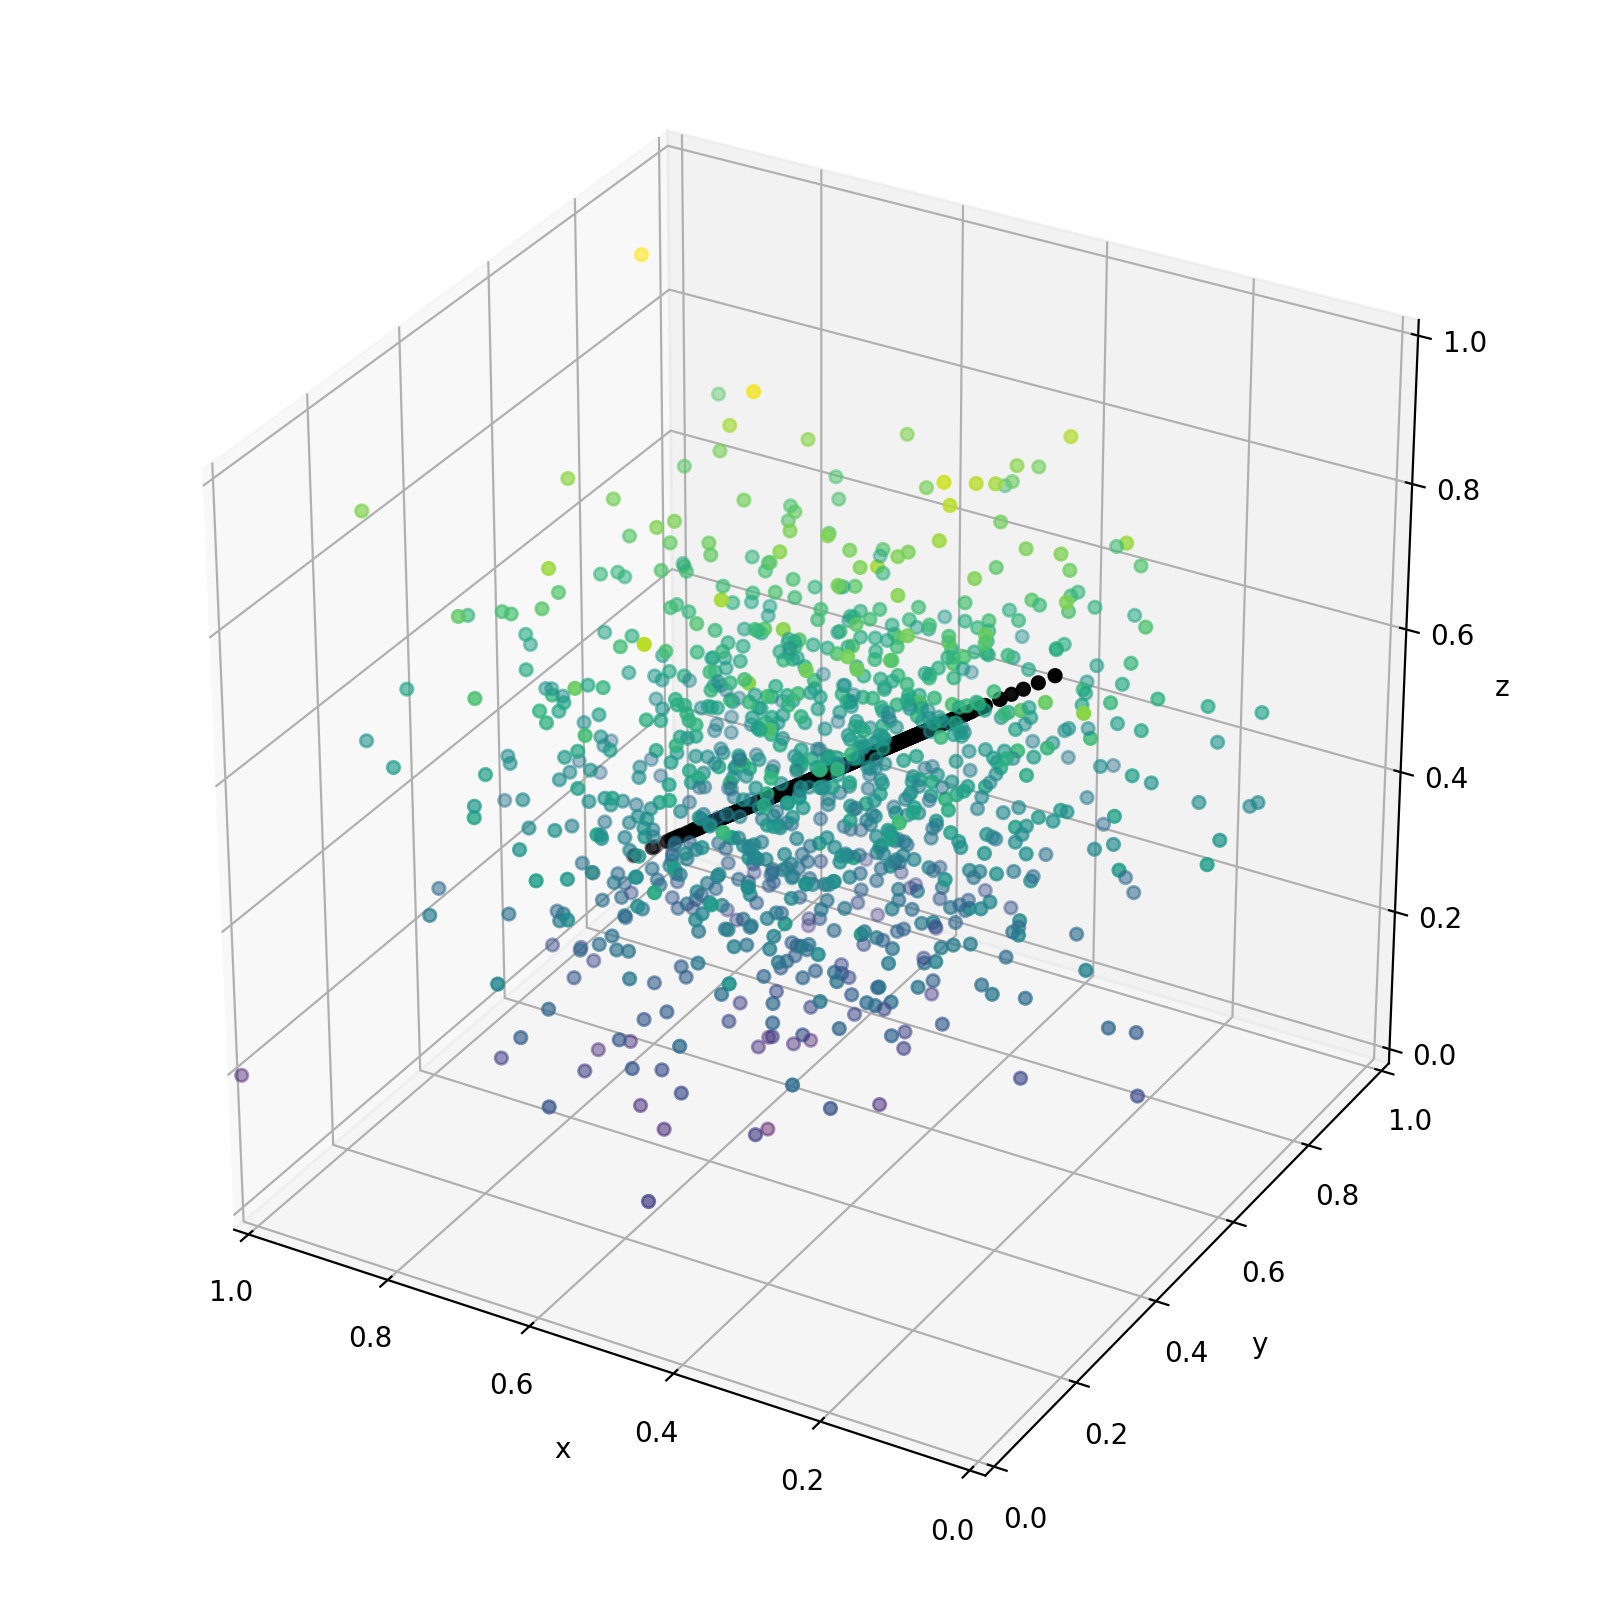
\includegraphics[width=\linewidth]{resources/X_Y_1_simulated.png}
			\caption{$\xx, \yy; \; t=1$}
			\label{fig:1}
		\end{subfigure}\hfil
		\begin{subfigure}{0.2\textwidth}
			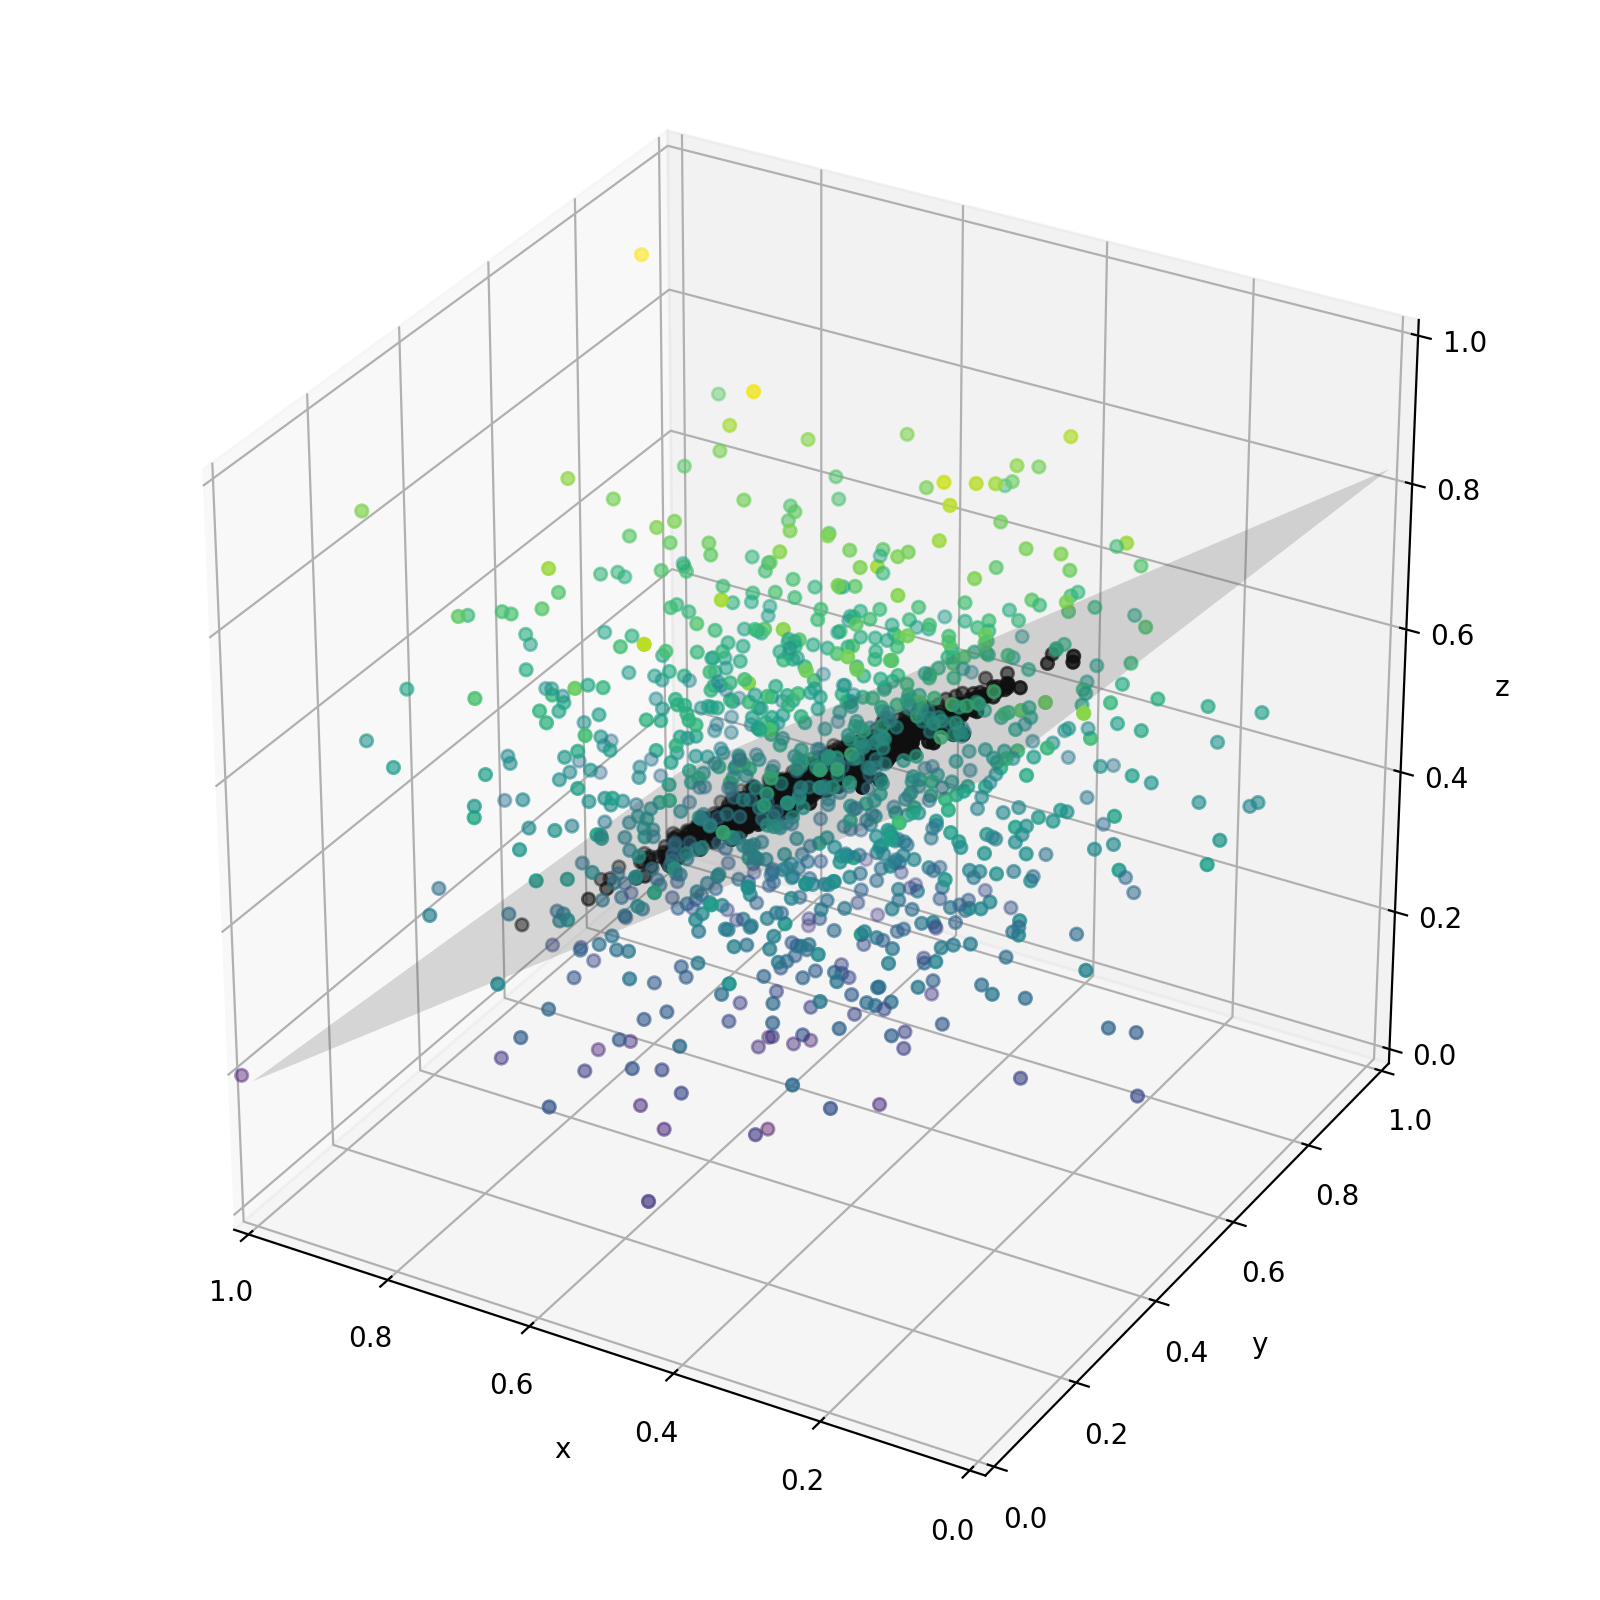
\includegraphics[width=\linewidth]{resources/X_Y_2_simulated.png}
			\caption{$\xx, \yy; \; t=2$}
			\label{fig:2}
		\end{subfigure}\hfil
		\begin{subfigure}{0.2\textwidth}
			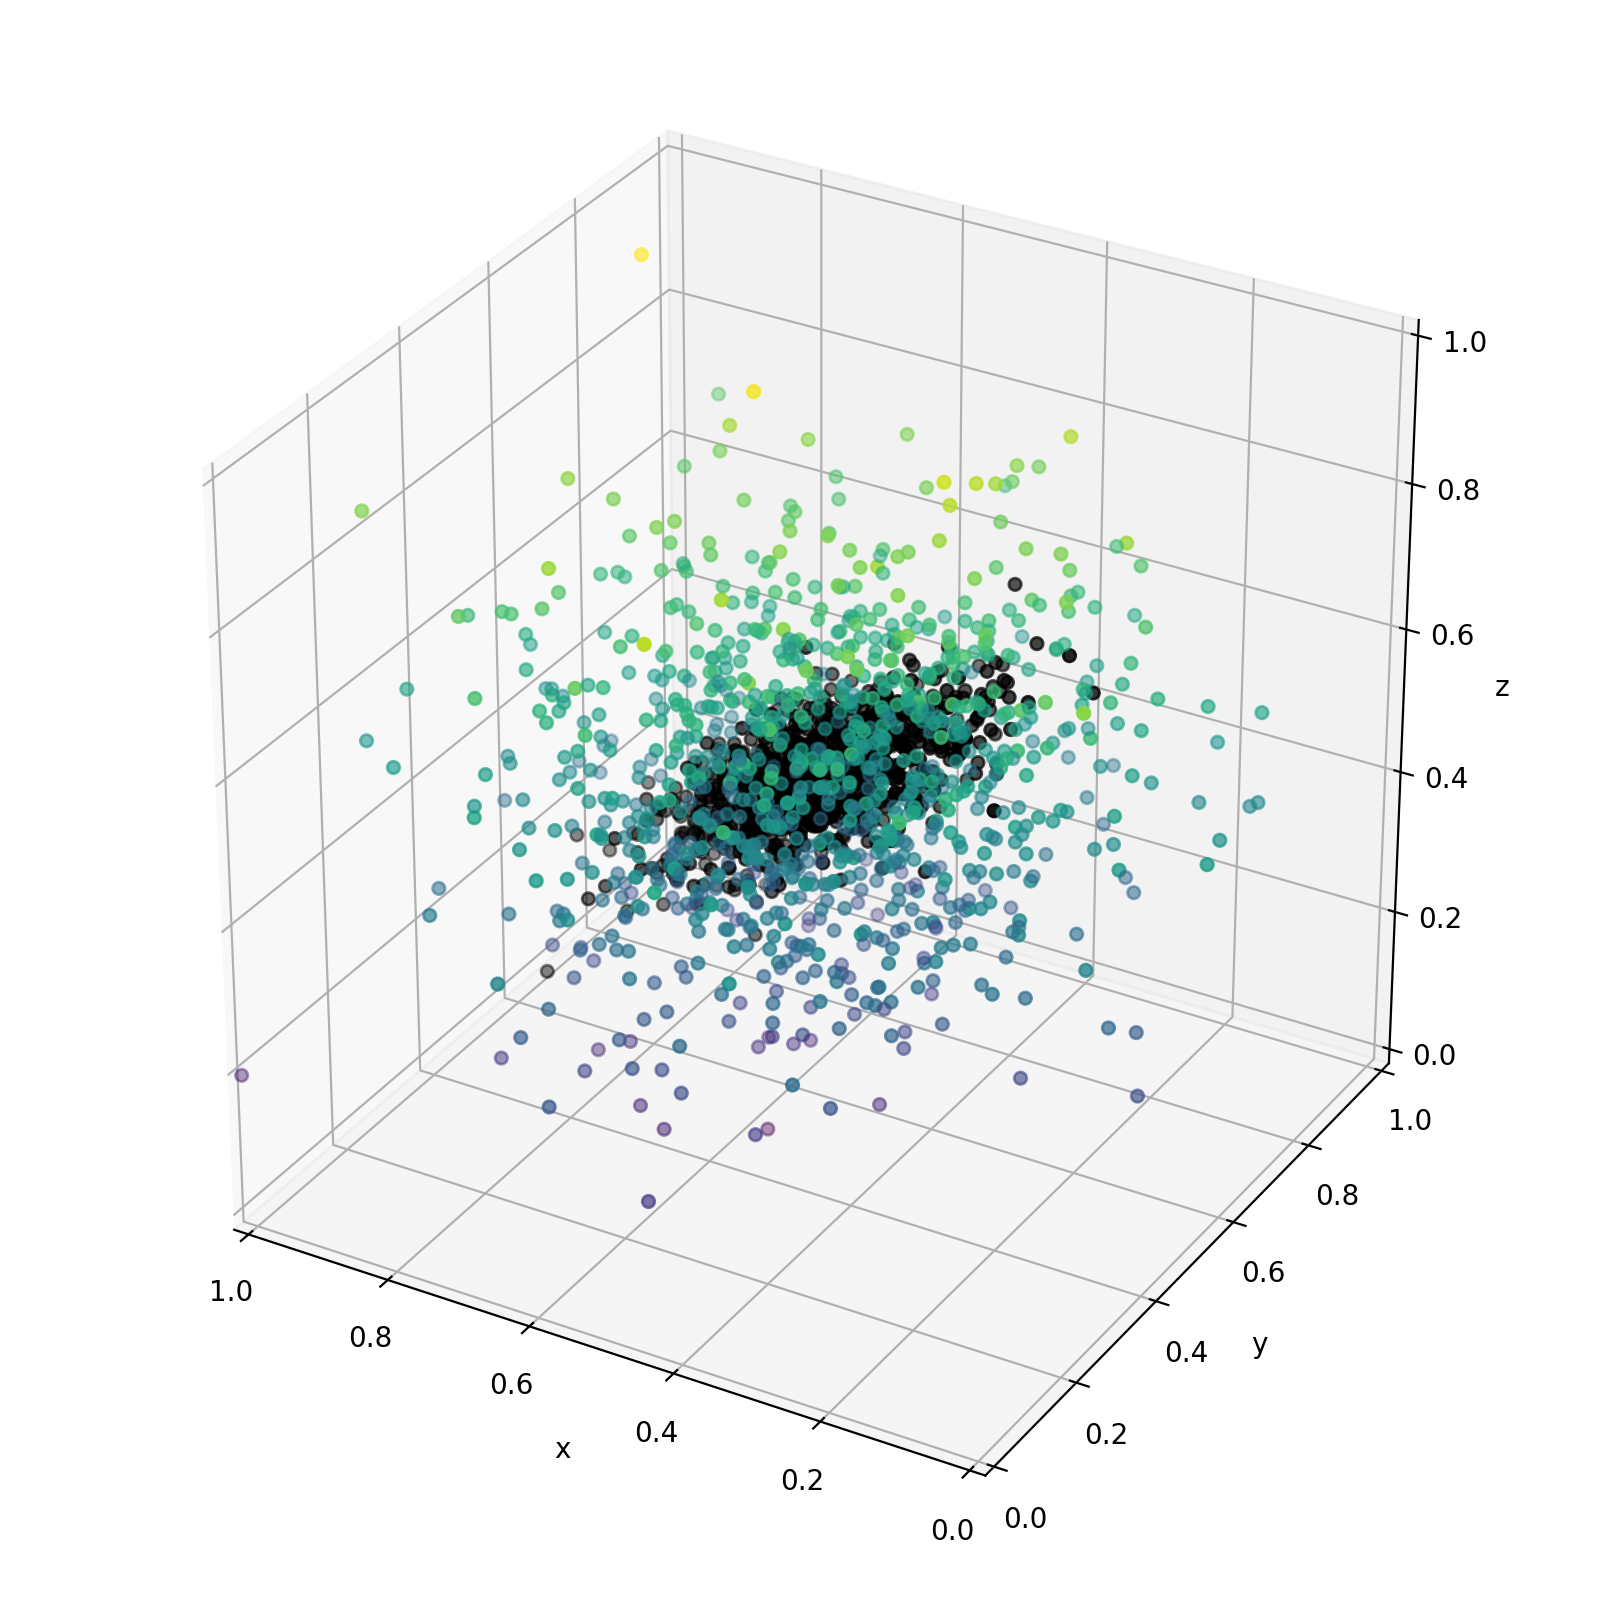
\includegraphics[width=\linewidth]{resources/X_Y_3_simulated.png}
			\caption{$\xx, \yy; \; t=3$}
			\label{fig:3}
		\end{subfigure}
		
		\medskip
		\begin{subfigure}{0.2\textwidth}
			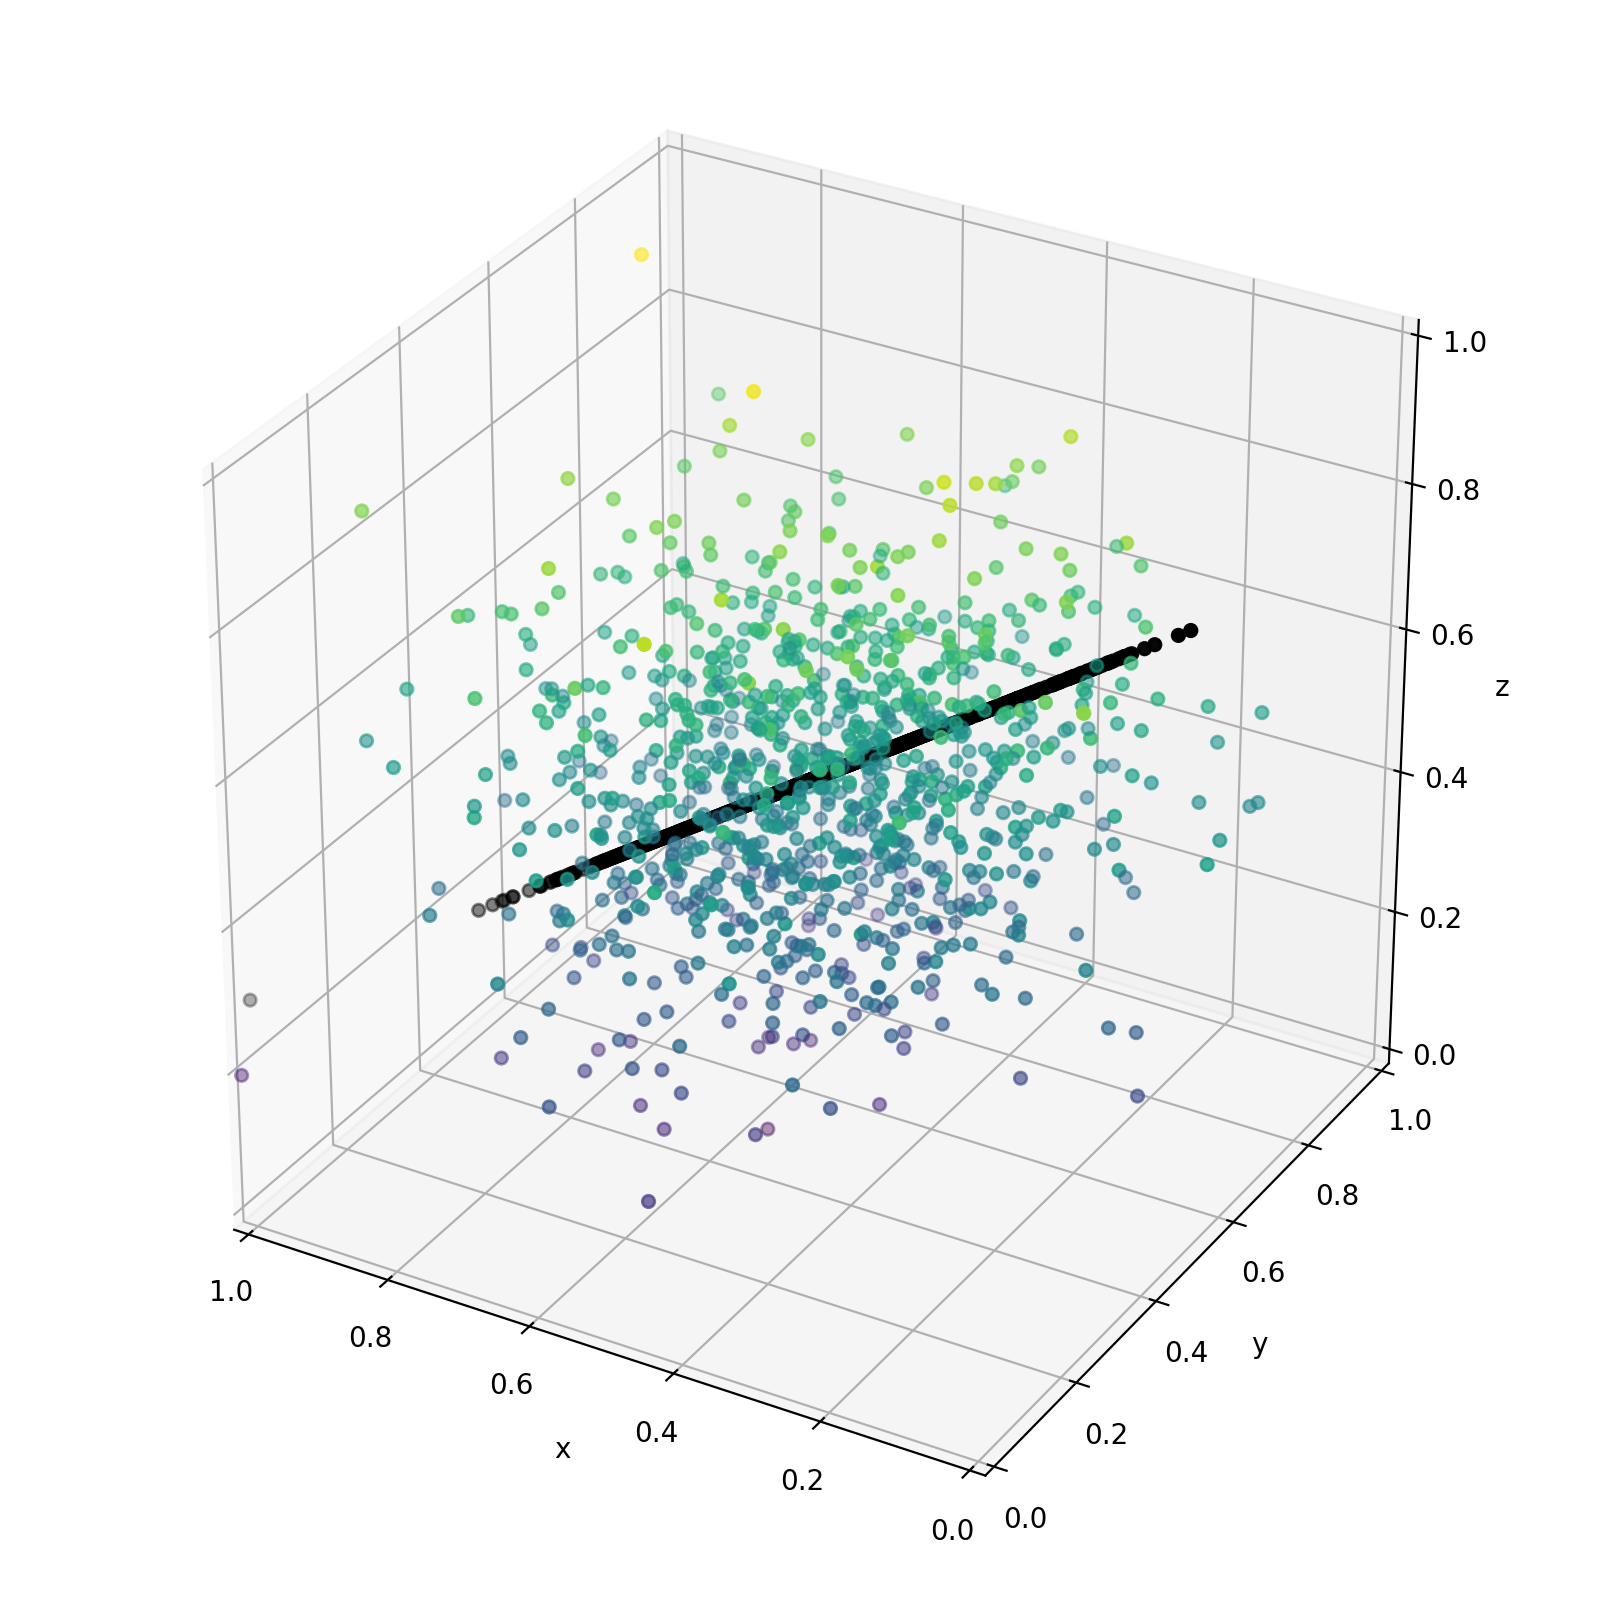
\includegraphics[width=\linewidth]{resources/Y_Y_1_simulated.png}
			\caption{$\yy, \yy; \; t=1$}
			\label{fig:4}
		\end{subfigure}\hfil
		\begin{subfigure}{0.2\textwidth}
			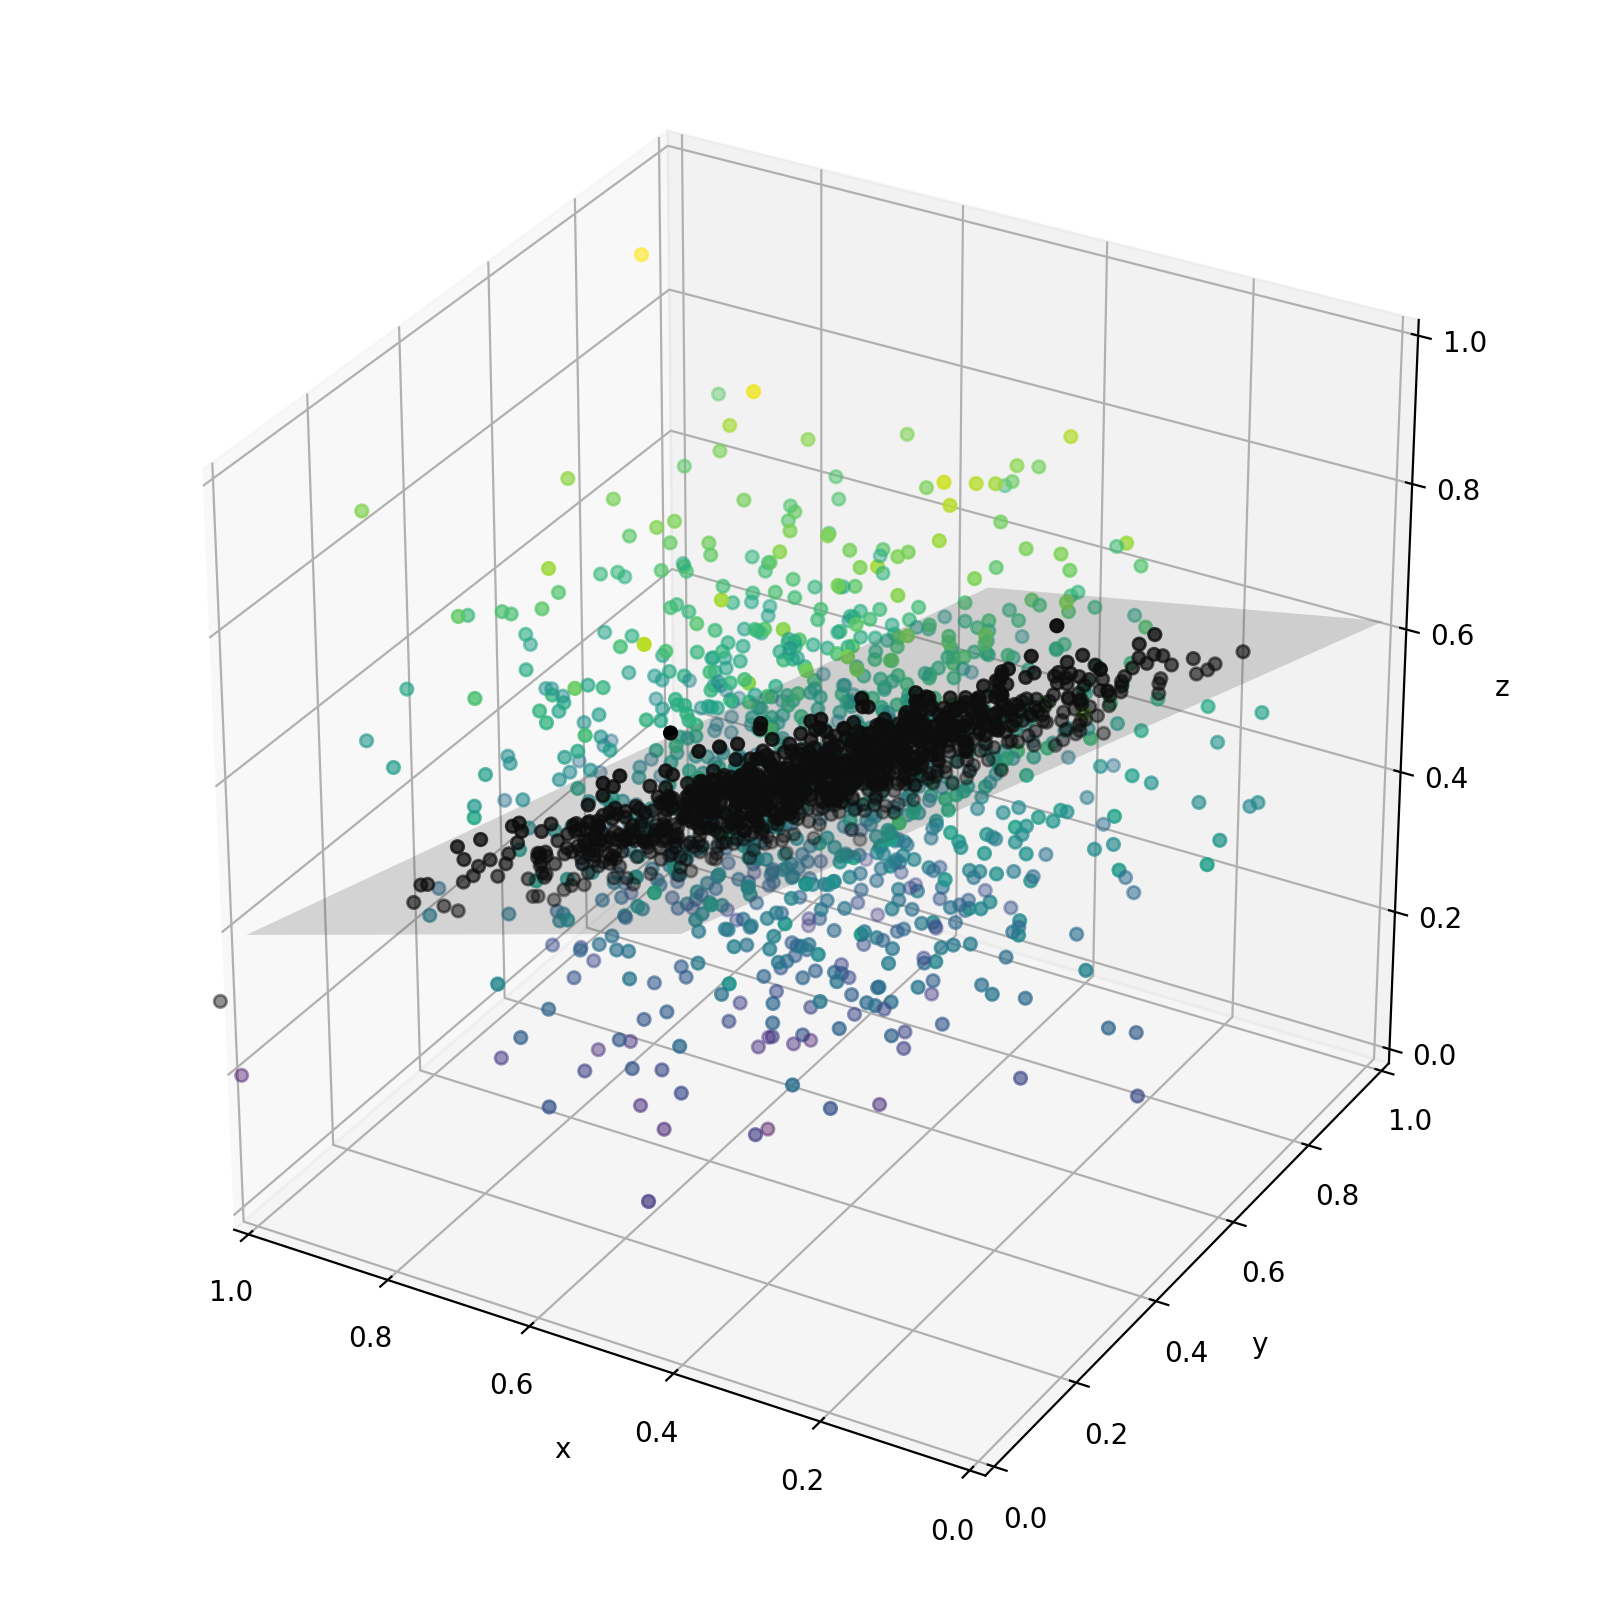
\includegraphics[width=\linewidth]{resources/Y_Y_2_simulated.png}
			\caption{$\yy, \yy; \; t=2$}
			\label{fig:5}
		\end{subfigure}\hfil
		\begin{subfigure}{0.2\textwidth}
			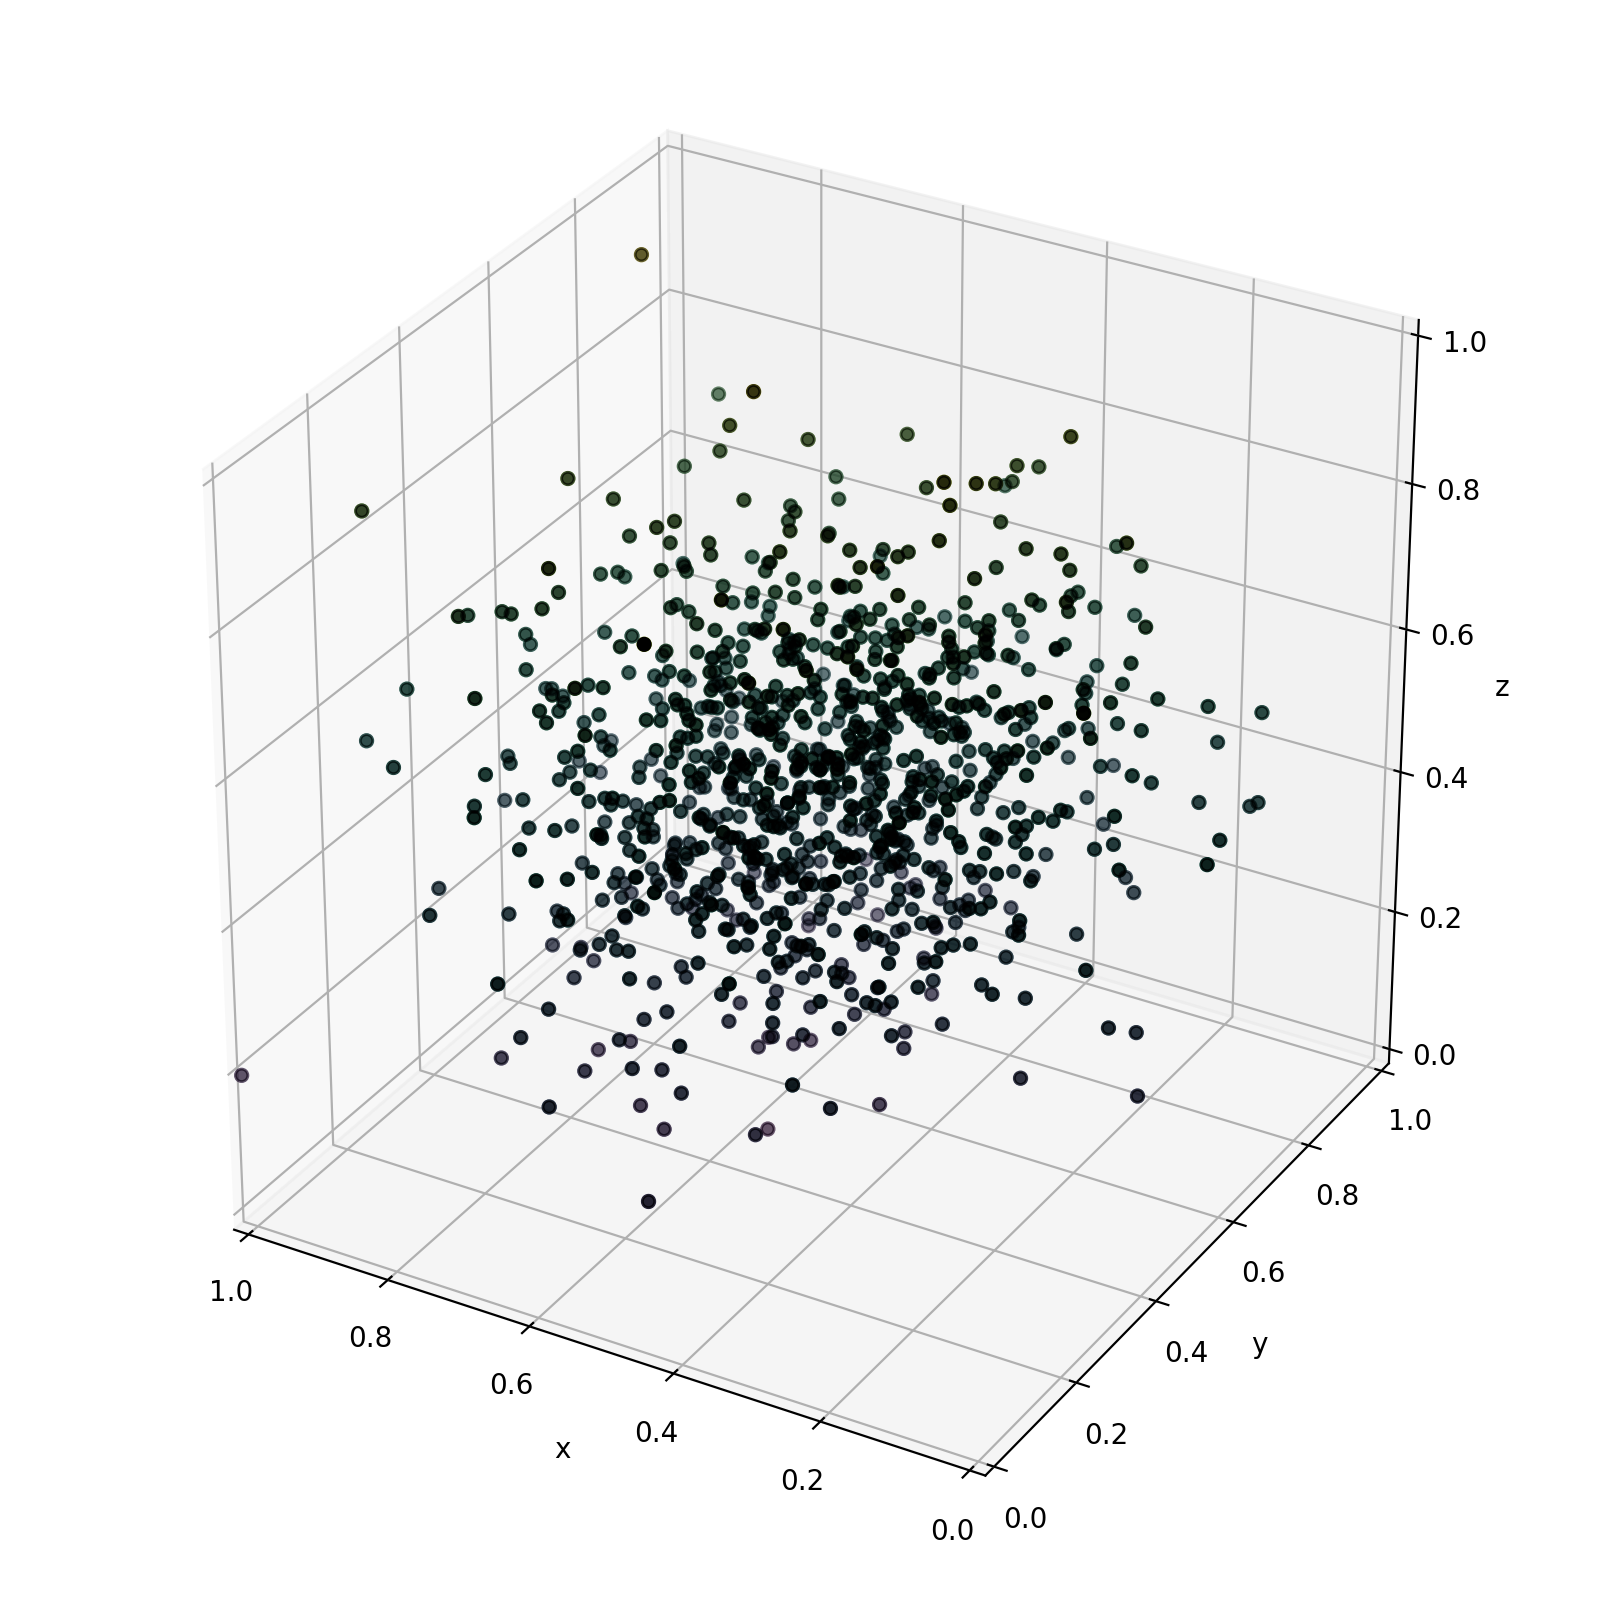
\includegraphics[width=\linewidth]{resources/Y_Y_3_simulated.png}
			\caption{$\yy, \yy; \; t=3$}
			\label{fig:6}
		\end{subfigure}
	\end{figure}
\end{frame}

\begin{frame}{Effektive Dimension der Regression}
\begin{alertblock}{}
	\begin{center}
		Reduced-Rank-Regressionsmodell: $ \qquad \Y = \muu + \C \X + \mathcal{E}\text{,} \quad  \rk \,\C \leq t $
	\end{center}
\end{alertblock}
\begin{alertblock}{}
	\begin{center}
		Haben zuvor $ W_{t, \Ggamma}(\muu, \C) := \E[(\Y - \muu - \C \X)^{\top} \Ggamma (\Y - \muu - \C \X)]$ minimiert
	\end{center}
\end{alertblock}
	Wie wählt man die \textit{effektive Dimension} $t$ bei der Reduced-Rank-Regression geeignet? 
	
	Vergrößert man den Rang von $\C$ von $t = t_0$ zu $t = t_1$, $\; t_0 < t_1$, so
	$$W_{t_0, \Ggamma}(\muu^{(t_0)}_{\min}, \A^{(t_0)}_{\min}, \B^{(t_0)}_{\min}) - W_{t_1, \Ggamma}(\muu^{(t_1)}_{\min}, \A^{(t_1)}_{\min}, \B^{(t_1)}_{\min}) = \sum_{i=t_0+1}^{t_1} \lambda_i$$
	wobei $\lambda_1 \geq \dots \geq \lambda_t \geq 0$ Eigenwerte von $\Ggamma^{1/2} \Ssigma_{\Y\X} \Ssigma_{\X\X}^{-1} \Ssigma_{\X\Y} \Ggamma^{1/2}$ nach Größe sortiert.
	
	\begin{itemize}
		\item In der Praxis (mit $\widehat{\lambda}_i$) untersuchen, bis wann es sich \glqq lohnt\grqq , $t$ zu vergrößern
		\item etwa mit Tests, ob $\rk \, \Ggamma^{1/2} \Ssigma_{\Y\X} \Ssigma_{\X\X}^{-1} \Ssigma_{\X\Y} \Ggamma^{1/2} = \rk \, \Ssigma_{\Y\X}$ kleiner als eine festgelegte Zahl ist
	\end{itemize}
\end{frame}

\begin{frame}
	\begin{center}
		\large Vielen Dank für Ihre Aufmerksamkeit.
	\end{center}
\end{frame}
\end{document}
